\documentclass[11pt,a4paper]{article}

\usepackage[utf8]{inputenc}
\usepackage[T1]{fontenc}
\usepackage[a4paper,margin=2.5cm]{geometry}
\usepackage{amsmath,amssymb}
\usepackage{graphicx}
\usepackage{booktabs}
\usepackage{enumitem}
\usepackage{hyperref}
\usepackage{xcolor}
\usepackage{fancyhdr}
\usepackage{titlesec}
\usepackage{listings}

\hypersetup{colorlinks=true,linkcolor=blue!50!black,citecolor=blue!50!black,urlcolor=blue!50!black}
\titleformat{\section}{\normalfont\Large\bfseries}{\thesection}{1em}{}
\titleformat{\subsection}{\normalfont\large\bfseries}{\thesubsection}{1em}{}

\definecolor{codebg}{RGB}{245,245,245}
\definecolor{codekw}{RGB}{0,80,150}
\definecolor{codecomment}{RGB}{110,110,110}
\lstset{
  backgroundcolor=\color{codebg},
  basicstyle=\ttfamily\small,
  keywordstyle=\color{codekw}\bfseries,
  commentstyle=\color{codecomment}\itshape,
  stringstyle=\color{teal},
  numbers=left, numberstyle=\tiny\color{gray}, numbersep=8pt,
  frame=single, framerule=0.3pt, rulecolor=\color{gray!40},
  breaklines=true, showstringspaces=false,
  language=Python, tabsize=2, xleftmargin=1.5em
}

\newcommand{\R}{\mathbb{R}}

\pagestyle{fancy}
\fancyhf{}
\rhead{\small Application SVD --- Courbe à terme WTI}
\lhead{\small Hippolyte Perraud}
\cfoot{\thepage}

\title{\vspace{-1.5cm}\textbf{PCA (via SVD) de la courbe des prix à terme du pétrole\\
\large Extraction des facteurs de risque niveau / pente / courbure}}
\author{Hippolyte Perraud \\ \small INSA Rouen Normandie -- Département Mathématiques Appliquées}
\date{\today}

\begin{document}
\maketitle
\thispagestyle{fancy}

\begin{abstract}
\noindent On applique ici la SVD à un problème concret de finance des matières premières : la décomposition de la dynamique de la courbe des prix à terme (\emph{term structure}) du pétrole WTI en un petit nombre de facteurs de risque interprétables -- niveau, pente et courbure -- selon une approche classique de desk de trading (dans l'esprit de Litterman--Scheinkman). L'analyse est menée sur des données réelles et publiques de l'\emph{U.S. Energy Information Administration} (EIA), portant sur les contrats à terme WTI 1 à 4 mois, de janvier 1985 à avril 2024. Ce travail complète, par une approche linéaire et classique, le projet de fin d'études sur les modèles de diffusion et de \emph{flow matching} appliqués à la même famille de données.
\end{abstract}

\section{Contexte et objectif}

Sur un desk de trading de matières premières, la courbe des prix à terme (le prix de contrats de maturités différentes à un instant donné) ne bouge presque jamais de façon totalement libre : ses déformations dans le temps sont très majoritairement decrites par un petit nombre de mouvements caractéristiques. L'approche standard, historiquement développée pour les courbes de taux d'intérêt (Litterman et Scheinkman, 1991) et transposée telle quelle aux courbes de matières premières, consiste à effectuer une analyse en composantes principales (PCA) des variations de la courbe, ce qui revient, comme vu dans le résumé théorique, à calculer la SVD de la matrice des variations centrées. On en tire typiquement trois facteurs dominants :
\begin{itemize}[nosep]
    \item le \textbf{niveau} : toute la courbe monte ou descend en bloc ;
    \item la \textbf{pente} : la courbe s'aplatit ou se pentifie (évolution du \emph{contango}/\emph{backwardation}) ;
    \item la \textbf{courbure} : le milieu de la courbe se déforme par rapport à ses extrémités.
\end{itemize}
Ces facteurs sont utilisés en pratique pour la couverture de portefeuille (combien de contrats de chaque maturité pour être neutre à un choc de niveau, de pente\ldots) et pour la simulation de scénarios de risque.

\section{Données}

Les données utilisées sont les prix de règlement mensuels des contrats à terme \emph{light sweet crude oil} (WTI), livrables à Cushing, Oklahoma, sur le NYMEX, pour les échéances 1 à 4 mois (séries \texttt{RCLC1} à \texttt{RCLC4}), publiées par l'EIA\footnote{\url{https://www.eia.gov/dnav/pet/pet_pri_fut_s1_m.htm}}. La série couvre \textbf{472 mois}, de janvier 1985 à avril 2024 -- l'EIA ayant cessé la mise à jour de cette série après le 5 avril 2024, comme l'indique explicitement la page source. Il s'agit donc d'un panel réel et public, sans aucune donnée simulée.

Pour un mois donné, la courbe observée est le vecteur $(F^{(1)}_t, F^{(2)}_t, F^{(3)}_t, F^{(4)}_t)$ des quatre prix à terme. La matrice de données est donc $X \in \R^{472 \times 4}$ : $n=472$ dates (les "snapshots" de la Section 2 du résumé théorique) et $m=4$ maturités.

\section{Méthodologie}

Conformément à la pratique de desk, la PCA est menée non pas sur les niveaux de prix (fortement non stationnaires) mais sur les \textbf{variations mensuelles} de la courbe, $\Delta X_t = X_t - X_{t-1} \in \R^{4}$, empilées dans une matrice $\Delta X \in \R^{471 \times 4}$. On centre chaque colonne (soustraction de la moyenne), puis on calcule la SVD de la matrice centrée :
\begin{equation}
\Delta X_{\text{centré}} = U \Sigma V^{\top}, \qquad U \in \R^{471\times 4},\ \Sigma \in \R^{4\times4},\ V \in \R^{4\times 4}.
\end{equation}
Comme rappelé dans le résumé théorique (Section 6), les colonnes de $V$ sont exactement les composantes principales : ce sont les vecteurs propres de la matrice de covariance des variations $\frac{1}{n-1}\Delta X_{\text{centré}}^{\top}\Delta X_{\text{centré}}$, et les valeurs singulières au carré, normalisées par leur somme, donnent la part de variance expliquée par chaque facteur. Le premier vecteur colonne de $V$ (associé à la plus grande valeur singulière) est le facteur de \emph{niveau}, le second la \emph{pente}, le troisième la \emph{courbure} -- ces noms étant justifiés a posteriori par la forme des vecteurs obtenus (Section~\ref{sec:resultats}), et non imposés a priori.

\section{Code}

L'analyse est entièrement reproduite en Python (NumPy/Pandas), à partir du panel de 472 lignes ci-dessus. Le cœur du calcul se résume aux quelques lignes suivantes (le prétraitement des données brutes EIA est omis par souci de concision) :

\begin{lstlisting}[caption={SVD de la matrice des variations de la courbe WTI}, label={lst:svd}]
import numpy as np
import pandas as pd

panel = pd.read_csv("wti_curve_panel.csv", parse_dates=["date"])
maturities = ["C1", "C2", "C3", "C4"]      # contrats a 1..4 mois
X = panel[maturities].to_numpy()           # (472, 4), $/baril

# Variations mensuelles de la courbe puis centrage
dX = np.diff(X, axis=0)                    # (471, 4)
dX_centered = dX - dX.mean(axis=0)

# SVD -> facteurs de risque de la courbe
U, S, Vt = np.linalg.svd(dX_centered, full_matrices=False)
V = Vt.T                                   # colonnes = niveau, pente, courbure...

explained_var = (S**2) / np.sum(S**2)      # variance expliquee par facteur
scores = dX_centered @ V                   # score (choc) de chaque facteur, par mois
\end{lstlisting}

Le code complet (préparation des données, figures, export des résultats) est fourni en archive avec ce document.

\section{Résultats}
\label{sec:resultats}

\subsection{Variance expliquée}

Le Tableau~\ref{tab:variance} et la Figure~\ref{fig:variance} montrent que le premier facteur (niveau) explique à lui seul \textbf{99,16\,\%} de la variance des variations mensuelles de la courbe -- un résultat attendu puisque des contrats de maturités aussi rapprochées (1 à 4 mois) sont extrêmement corrélés entre eux. Les facteurs de pente et de courbure, bien que ne représentant que 0,81\,\% et 0,04\,\% de la variance, restent économiquement significatifs : ce sont eux qui pilotent les écarts entre maturités, donc le risque de \emph{spread}, alors qu'un simple hedge en niveau (une seule quantité de contrats, indépendamment de la maturité) laisse ce risque totalement découvert.

\begin{table}[h]
\centering
\begin{tabular}{lcccc}
\toprule
Facteur & Valeur singulière & Variance expliquée & Variance cumulée \\
\midrule
1 -- Niveau     & 188,16 & 99,16\,\% & 99,16\,\%  \\
2 -- Pente      & 16,97  & 0,81\,\%  & 99,96\,\%  \\
3 -- Courbure   & 3,54   & 0,04\,\%  & 100,00\,\% \\
4 -- (résiduel) & 0,67   & 0,00\,\%  & 100,00\,\% \\
\bottomrule
\end{tabular}
\caption{Décomposition en valeurs singulières des variations mensuelles de la courbe WTI (1985--2024).}
\label{tab:variance}
\end{table}

\begin{figure}[h]
\centering
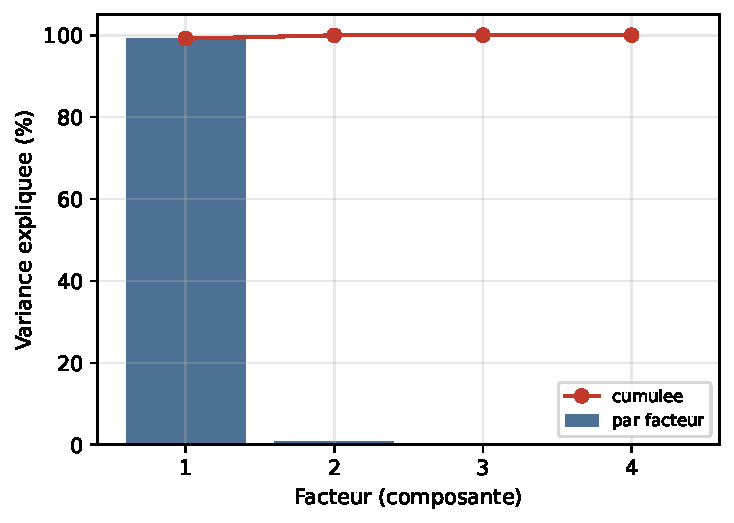
\includegraphics[width=0.7\textwidth]{figures/pca_variance.pdf}
\caption{Variance expliquée par facteur et variance cumulée.}
\label{fig:variance}
\end{figure}

\subsection{Forme des facteurs : niveau, pente, courbure}

La Figure~\ref{fig:loadings} affiche les coefficients (\emph{loadings}) des trois premiers vecteurs de $V$ en fonction de la maturité. Leur forme confirme l'interprétation classique :
\begin{itemize}[nosep]
    \item le facteur 1 a des coefficients tous positifs et proches (0,53 à 0,47) : un choc sur ce facteur déplace quasiment en bloc les quatre maturités -- c'est bien un facteur de \textbf{niveau} ;
    \item le facteur 2 est croissant avec la maturité, de $-0,75$ (contrat 1) à $+0,57$ (contrat 4) : un choc positif aplatit la courbe (fait monter les maturités longues relativement aux courtes) -- c'est la \textbf{pente} ;
    \item le facteur 3 change deux fois de signe (positif, négatif, négatif, positif) : c'est la signature classique d'un facteur de \textbf{courbure}, qui déforme le milieu de la courbe par rapport à ses extrémités.
\end{itemize}

\begin{figure}[h]
\centering
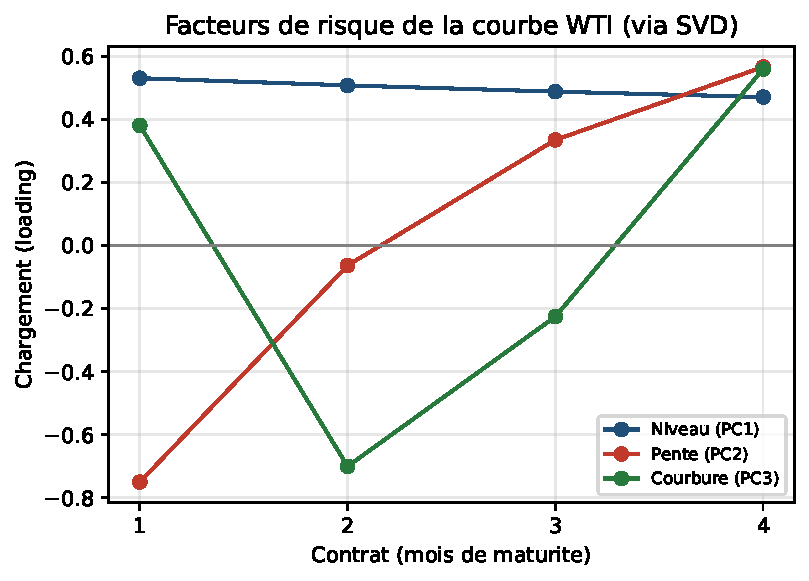
\includegraphics[width=0.7\textwidth]{figures/pca_loadings.pdf}
\caption{Coefficients (\emph{loadings}) des trois premiers facteurs en fonction de la maturité.}
\label{fig:loadings}
\end{figure}

La Figure~\ref{fig:shocks} illustre concrètement l'effet d'un choc de $\pm 1$ écart-type sur chacun des deux premiers facteurs, appliqué à la courbe moyenne observée sur la période : le choc de niveau translate la courbe, le choc de pente la fait pivoter.

\begin{figure}[h]
\centering
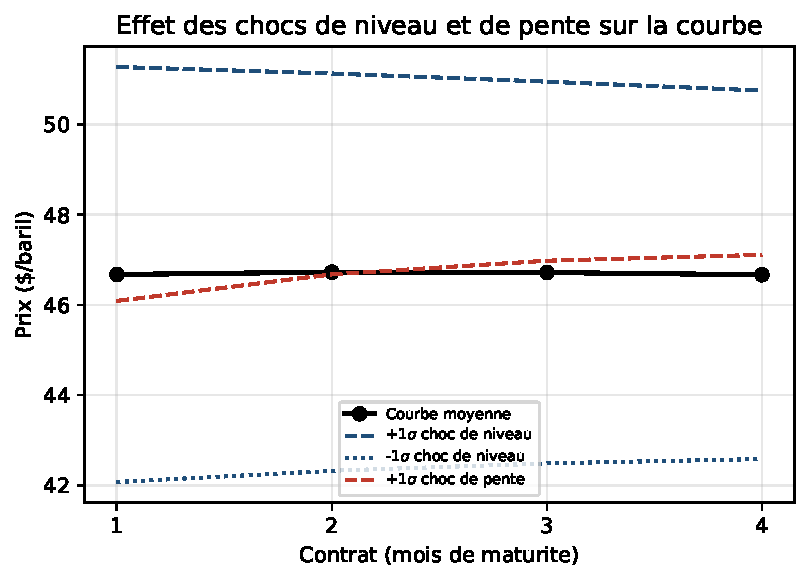
\includegraphics[width=0.68\textwidth]{figures/pca_curve_shocks.pdf}
\caption{Courbe moyenne 1985--2024 et effet d'un choc de $\pm 1\sigma$ sur les facteurs de niveau et de pente.}
\label{fig:shocks}
\end{figure}

\subsection{Lecture économique dans le temps}

La Figure~\ref{fig:spread} trace, non pas le facteur de pente lui-même, mais son pendant direct et interprétable en dollars : l'écart entre le contrat à 4 mois et le contrat à 1 mois, $F^{(4)}_t - F^{(1)}_t$. On y reconnaît sans ambiguïté les grands épisodes de marché : le \emph{contango} prononcé de la crise de 2008--2009 et du choc de demande de 2015--2016 (accumulation de stocks, marché en surplus), et surtout le pic extrême d'avril 2020, lorsque la saturation des capacités de stockage à Cushing a provoqué le passage du contrat front-month en territoire négatif -- un épisode que l'on retrouve exactement à la même date dans le score du facteur de pente proprement dit (Figure~\ref{fig:slope}), qui atteint son extremum sur toute la période étudiée.

\begin{figure}[h]
\centering
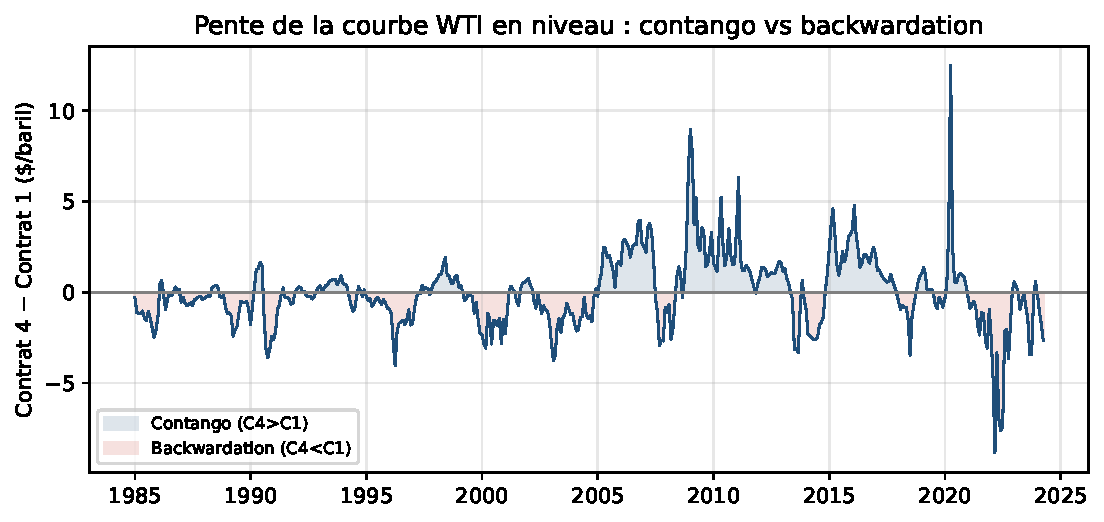
\includegraphics[width=0.85\textwidth]{figures/pca_level_vs_price.pdf}
\caption{Écart Contrat 4 $-$ Contrat 1 : contango (bleu) vs backwardation (rouge).}
\label{fig:spread}
\end{figure}

\begin{figure}[h]
\centering
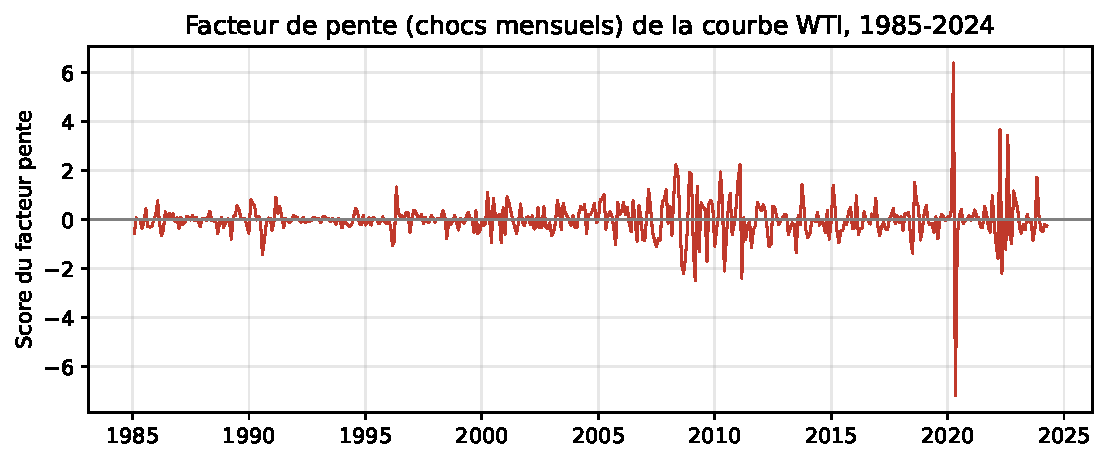
\includegraphics[width=0.85\textwidth]{figures/pca_slope_timeseries.pdf}
\caption{Score mensuel du facteur de pente (deuxième composante de la SVD).}
\label{fig:slope}
\end{figure}

\section{Discussion et limites}

Cette étude illustre, sur un cas réel, l'ensemble de la chaîne théorique décrite dans le résumé d'article : la SVD comme outil de PCA (Section~6 du résumé), le théorème d'Eckart--Young qui garantit qu'un modèle à 2 ou 3 facteurs est la meilleure approximation possible de la dynamique de la courbe à ce rang (Section~4), et l'interprétation géométrique des facteurs comme axes principaux de l'ellipsoïde des variations de la courbe (Section~3.2).

Deux limites méritent d'être soulignées. D'une part, ne disposer que de quatre maturités (1 à 4 mois) restreint la résolution du facteur de courbure, qui serait mieux identifié avec une courbe plus riche (par exemple 12 ou 24 points, comme le permettent les données CME complètes, mais qui ne sont pas librement accessibles). D'autre part, la SVD est par construction une méthode \emph{linéaire} : elle ne capture que des déformations de la courbe qui sont des combinaisons linéaires fixes des maturités, alors que la dynamique réelle des marchés de matières premières -- en particulier lors d'épisodes extrêmes comme avril 2020 -- comporte des non-linéarités que seule une approche de type diffusion ou \emph{flow matching}, comme dans le projet de fin d'études, peut chercher à capturer. Les deux approches sont donc complémentaires : la SVD donne une décomposition simple, interprétable et immédiatement exploitable pour la couverture ; les modèles génératifs visent une description plus fine, mais moins directement interprétable, de la dynamique complète de la courbe.

\section{Conclusion}

Sur des données réelles et publiques de l'EIA couvrant près de quarante ans de marché WTI, la SVD des variations mensuelles de la courbe à terme retrouve exactement la décomposition niveau/pente/courbure attendue par la théorie et la pratique de desk, avec un facteur de niveau expliquant plus de 99\,\% de la variance et des facteurs de pente et de courbure dont la dynamique correspond précisément aux épisodes de marché connus (crise de 2008, choc de 2020). Cette application concrète illustre la puissance et les limites d'un outil linéaire simple face à un problème de finance des matières premières.

\end{document}
